\documentclass{beamer}
\usepackage{graphicx}
\usepackage{xcolor}
\usepackage{tikz}
\usepackage{amsmath}
\DeclareGraphicsExtensions{.png,.pdf,.jpg,.jpeg}

\definecolor{purpleblue}{RGB}{80, 80, 180}
\definecolor{lightgray}{RGB}{230, 230, 230}
\definecolor{novelPurple}{RGB}{98, 54, 255}
\definecolor{darkgray}{RGB}{50, 50, 50}
\definecolor{softPurple}{RGB}{180, 170, 255}
\definecolor{softGray}{RGB}{235, 235, 245}
\definecolor{lightText}{RGB}{90, 90, 110}
\graphicspath{{static/unit4/}{./}}

\usetheme{Madrid}
\usecolortheme{dolphin}

\setbeamerfont{title}{size=\Large,series=\bfseries}
\setbeamerfont{frametitle}{size=\LARGE,series=\bfseries}
\setbeamercolor{frametitle}{fg=white, bg=novelPurple}
\setbeamercolor{title}{fg=white, bg=purpleblue}

\title[SAT Unit 4.3]{\textbf{SAT Unit 4.3 \\Trigonometry}}
\author{\textbf{Jack Zeng}}
\institute{\textcolor{white}{\textbf{Novel Prep}}}
\date{\today}

\begin{document}

\begin{frame}
    \titlepage
    \vfill
    \begin{flushright}
        \textcolor{purpleblue}{\Huge \textbf{Novel Prep}}
    \end{flushright}
\end{frame}

\begin{frame}
    \begin{tikzpicture}[remember picture, overlay]
        \shade[top color=softPurple, bottom color=softGray]
            (current page.north west) rectangle (current page.south east);
        \fill[white, opacity=0.3] (current page.center) circle (4cm);
        \node[align=center] at (current page.center) {
            {\Huge\bfseries\textcolor{purpleblue}{Novel Prep}} \\[0.5cm]
            {\Large\itshape\textcolor{lightText}{Excellence in SAT Prep}}
        };
        \foreach \x in {1,2,3,4,5} {
            \fill[purpleblue, opacity=0.2] (rand*10-5, rand*7-3.5) circle (0.1+\x*0.05);
        }
    \end{tikzpicture}
\end{frame}

\begin{frame}{Overview}
    \tableofcontents
\end{frame}


\begin{frame}
\section{Trigonometric Ratios of Acute Angles}
    \begin{tikzpicture}[remember picture, overlay]
        \shade[top color=softPurple, bottom color=softGray]
            (current page.north west) rectangle (current page.south east);
        \fill[white, opacity=0.3] (current page.center) circle (4cm);
        \node[align=center] at (current page.center) {
            {\LARGE\bfseries\textcolor{purpleblue}{Trigonometric Ratios of Acute Angles}} \\[0.5cm]
            {\Large\itshape\textcolor{lightText}{Excellence in SAT Prep}}
        };
        \foreach \x in {1,2,3,4,5} {
            \fill[purpleblue, opacity=0.2] (rand*10-5, rand*7-3.5) circle (0.1+\x*0.05);
        }
    \end{tikzpicture}
\end{frame}


\begin{frame}{Right-Triangle Trigonometry}

For acute angle $\theta$ in a right triangle:
\[
\sin \theta = \frac{\text{opp}}{\text{hyp}}, \quad
\cos \theta = \frac{\text{adj}}{\text{hyp}}, \quad
\tan \theta = \frac{\text{opp}}{\text{adj}}
\]

\vspace{0.15cm}
\textbf{Special right triangles:}
\begin{itemize}
    \item $45^\circ$-$45^\circ$-$90^\circ$: sides $s,\ s,\ s\sqrt{2}$
    \item $30^\circ$-$60^\circ$-$90^\circ$: sides $s,\ s\sqrt{3},\ 2s$
\end{itemize}

\end{frame}

\begin{frame}{SOH-CAH-TOA}

\begin{itemize}
    \item \textbf{SOH:} $\sin\theta=\dfrac{\text{opposite}}{\text{hypotenuse}}$
    \item \textbf{CAH:} $\cos\theta=\dfrac{\text{adjacent}}{\text{hypotenuse}}$
    \item \textbf{TOA:} $\tan\theta=\dfrac{\text{opposite}}{\text{adjacent}}$
\end{itemize}

\vspace{0.2cm}
\textbf{SAT move:} label opposite, adjacent, and hypotenuse relative to the angle named in the problem.

\end{frame}

\begin{frame}{Special Right Triangles}

\textbf{$45^\circ$-$45^\circ$-$90^\circ$:}
\[
s,\quad s,\quad s\sqrt{2}
\]

\textbf{$30^\circ$-$60^\circ$-$90^\circ$:}
\[
s,\quad s\sqrt{3},\quad 2s
\]

\vspace{0.2cm}
\textbf{SAT move:} if an angle is $30^\circ$, $45^\circ$, or $60^\circ$, use the ratio before doing extra algebra.

\end{frame}

\begin{frame}{Complementary Angles}

In a right triangle, the two acute angles add to $90^\circ$.
\[
\sin A = \cos(90^\circ-A)
\]
\[
\tan A \cdot \tan(90^\circ-A)=1
\]

\vspace{0.2cm}
\textbf{Example:} If $\tan A=\dfrac{3}{4}$, then the tangent of the other acute angle is $\dfrac{4}{3}$.

\end{frame}

\begin{frame}{Similar Right Triangles}

If two right triangles share an acute angle, they are similar.

\vspace{0.2cm}
That means their trig ratios match:
\[
\sin A,\quad \cos A,\quad \tan A
\]
stay the same even if the triangle is scaled.

\vspace{0.2cm}
\textbf{SAT move:} do not solve every side if a trig ratio already gives the relationship.

\end{frame}

\begin{frame}{Worked Example: Tangent}

\textbf{Question:} In a right triangle, $\tan B=\dfrac{3}{4}$. What can the legs be?

\vspace{0.2cm}
\[
\tan B=\dfrac{\text{opposite}}{\text{adjacent}}=\dfrac{3}{4}
\]
So the legs are in the ratio $3:4$.

\vspace{0.2cm}
The hypotenuse is then in ratio $5$ by the $3$-$4$-$5$ triangle.

\end{frame}

\begin{frame}{Common Trig Traps}

\begin{itemize}
    \item Opposite and adjacent change when the named angle changes.
    \item The hypotenuse is always across from the right angle.
    \item $\tan$ never uses the hypotenuse.
    \item Similar triangles preserve trig ratios, not necessarily side lengths.
\end{itemize}

\end{frame}

\begin{frame}
\section{Radian Measure}
    \begin{tikzpicture}[remember picture, overlay]
        \shade[top color=softPurple, bottom color=softGray]
            (current page.north west) rectangle (current page.south east);
        \fill[white, opacity=0.3] (current page.center) circle (4cm);
        \node[align=center] at (current page.center) {
            {\LARGE\bfseries\textcolor{purpleblue}{Radian Measure}} \\[0.5cm]
            {\Large\itshape\textcolor{lightText}{Excellence in SAT Prep}}
        };
        \foreach \x in {1,2,3,4,5} {
            \fill[purpleblue, opacity=0.2] (rand*10-5, rand*7-3.5) circle (0.1+\x*0.05);
        }
    \end{tikzpicture}
\end{frame}


\begin{frame}{Understanding Radian Measure}
\textbf{Definition:} one radian is the angle created when arc length equals radius.
\[
\theta=\dfrac{s}{r}
\]
where $s$ is arc length and $r$ is radius.

\vspace{0.2cm}
\[
360^\circ=2\pi \text{ radians}
\]
\[
\theta_{\text{rad}}=\theta^\circ\cdot\dfrac{\pi}{180},
\qquad
\theta^\circ=\theta_{\text{rad}}\cdot\dfrac{180}{\pi}
\]
\end{frame}

\begin{frame}{Common Degree-Radian Conversions}
\begin{center}
\begin{tabular}{c|c}
Degrees & Radians \\
\hline
$30^\circ$ & $\dfrac{\pi}{6}$ \\
$45^\circ$ & $\dfrac{\pi}{4}$ \\
$60^\circ$ & $\dfrac{\pi}{3}$ \\
$90^\circ$ & $\dfrac{\pi}{2}$ \\
$180^\circ$ & $\pi$ \\
$360^\circ$ & $2\pi$
\end{tabular}
\end{center}
\end{frame}

\begin{frame}
\section{Trigonometric In Unit Circle}
    \begin{tikzpicture}[remember picture, overlay]
        \shade[top color=softPurple, bottom color=softGray]
            (current page.north west) rectangle (current page.south east);
        \fill[white, opacity=0.3] (current page.center) circle (4cm);
        \node[align=center] at (current page.center) {
            {\LARGE\bfseries\textcolor{purpleblue}{Trigonometric In Unit Circle}} \\[0.5cm]
            {\Large\itshape\textcolor{lightText}{Excellence in SAT Prep}}
        };
        \foreach \x in {1,2,3,4,5} {
            \fill[purpleblue, opacity=0.2] (rand*10-5, rand*7-3.5) circle (0.1+\x*0.05);
        }
    \end{tikzpicture}
\end{frame}


\begin{frame}{Trigonometric Ratios in the Unit Circle}
On the unit circle, a point at angle $\theta$ has coordinates:
\[
(\cos\theta,\ \sin\theta)
\]

\vspace{0.2cm}
\[
\tan\theta=\dfrac{\sin\theta}{\cos\theta}
\]

\textbf{SAT move:} connect right-triangle ratios to unit-circle coordinates.
\end{frame}

\begin{frame}
\section{Practice}
    \begin{tikzpicture}[remember picture, overlay]
        \shade[top color=softPurple, bottom color=softGray]
            (current page.north west) rectangle (current page.south east);
        \fill[white, opacity=0.3] (current page.center) circle (4cm);
        \node[align=center] at (current page.center) {
            {\LARGE\bfseries\textcolor{purpleblue}{Practice}} \\[0.5cm]
            {\Large\itshape\textcolor{lightText}{Excellence in SAT Prep}}
        };
        \foreach \x in {1,2,3,4,5} {
            \fill[purpleblue, opacity=0.2] (rand*10-5, rand*7-3.5) circle (0.1+\x*0.05);
        }
    \end{tikzpicture}
\end{frame}

\begin{frame}{Question: Triangle ABC above is a right triangle, and (B) = 5/13}
Triangle $ABC$ above is a right triangle, and $\sin(B) = \dfrac{5}{13}$.  
What is the length of side $\overline{BC}$?

\begin{center}
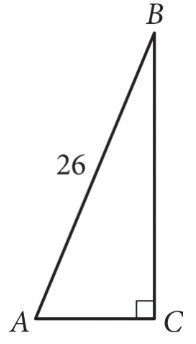
\includegraphics[width=0.48\linewidth]{17.jpg}
\end{center}
\end{frame}
\begin{frame}{Answer: Triangle ABC above is a right triangle, and (B) = 5/13}
\textit{Strategy:} Right triangle: $\sin B=\dfrac{\text{opp}}{\text{hyp}}$; find the missing side.

\textbf{Solution:}
\[ \boxed{24} \]
\textbf{Correct Answer:} \( \boxed{24} \)

\end{frame}
\begin{frame}{Question: In the triangle shown, what is the value of x°?}
\begin{center}
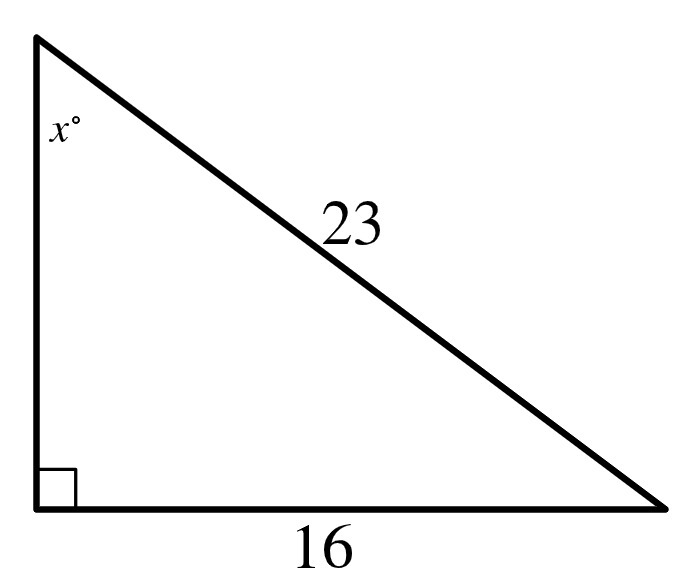
\includegraphics[width=0.52\linewidth]{18.jpg}
\end{center}

In the triangle shown, what is the value of $\sin x^\circ$?
\end{frame}
\begin{frame}{Answer: In the triangle shown, what is the value of x°?}
\textit{Strategy:} Label opposite/hypotenuse relative to angle $x$.

\textbf{Solution:}
\[ \boxed{6956} \]
\textit{Also accept: 6957, 16/23}
\textbf{Correct Answer:} \( \boxed{6956} \)

\end{frame}
\begin{frame}{Question: A graphic designer is creating a logo for a company. The logo is shown i…}
\begin{center}
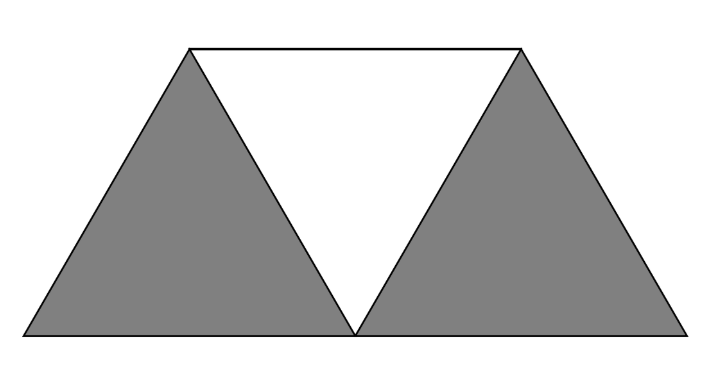
\includegraphics[width=0.54\linewidth]{19.png}
\end{center}

A graphic designer is creating a logo for a company. The logo is shown in the figure above. The logo is in the shape of a trapezoid and consists of three congruent equilateral triangles. If the perimeter of the logo is $20$ centimeters, what is the combined area of the shaded regions, in square centimeters, of the logo?
\begin{itemize}
    \item[\textbf{A.}] $2\sqrt{3}$
    \item[\textbf{B.}] $4\sqrt{3}$
    \item[\textbf{C.}] $8\sqrt{3}$
    \item[\textbf{D.}] $16$
\end{itemize}
\end{frame}
\begin{frame}{Answer: A graphic designer is creating a logo for a company. The logo is shown i…}
\textit{Strategy:} Equilateral triangles: height $=\dfrac{s\sqrt{3}}{2}$; shaded area from symmetry.

\textbf{Correct Answer:} \( \boxed{C} \)

\end{frame}
\begin{frame}{Question: The perimeter of an equilateral triangle is 624 centimeters. The height …}
The perimeter of an equilateral triangle is $624$ centimeters. The height of this triangle is $k\sqrt{3}$ centimeters, where $k$ is a constant. What is the value of $k$?
\end{frame}
\begin{frame}{Answer: The perimeter of an equilateral triangle is 624 centimeters. The height …}
\textit{Strategy:} Equilateral triangle side $=\dfrac{\text{perimeter}}{3}$; height $=\dfrac{s\sqrt{3}}{2}$.

\textbf{Solution:}
\[ \boxed{104} \]
\textbf{Correct Answer:} \( \boxed{104} \)

\end{frame}
\begin{frame}{Question: In the figure above, B = 3/4. If BC = 15 and DA = 4, what is the length …}
\begin{center}
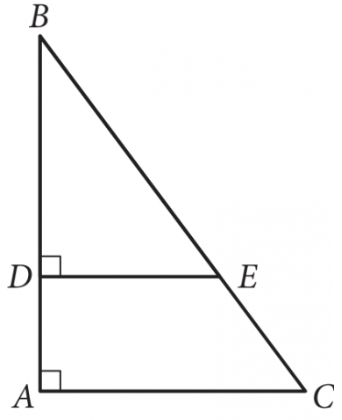
\includegraphics[width=0.52\linewidth]{20.png}
\end{center}

In the figure above, $\tan B = \dfrac{3}{4}$. If $BC = 15$ and $DA = 4$, what is the length of $\overline{DE}$?
\end{frame}
\begin{frame}{Answer: In the figure above, B = 3/4. If BC = 15 and DA = 4, what is the length …}
\textit{Strategy:} Use $\tan B=\dfrac{3}{4}$ to find missing legs, then similar triangles.

\textbf{Solution:}
\[ \boxed{6} \]
\textbf{Correct Answer:} \( \boxed{6} \)

\end{frame}
\begin{frame}{Question: An isosceles right triangle has a hypotenuse of length 58 inches. What i…}
An isosceles right triangle has a hypotenuse of length $58$ inches. What is the perimeter, in inches, of this triangle?
\begin{itemize}
    \item[\textbf{A.}] $29\sqrt{2}$
    \item[\textbf{B.}] $58\sqrt{2}$
    \item[\textbf{C.}] $58 + 58\sqrt{2}$
    \item[\textbf{D.}] $58 + 116\sqrt{2}$
\end{itemize}
\end{frame}
\begin{frame}{Answer: An isosceles right triangle has a hypotenuse of length 58 inches. What i…}
\textit{Strategy:} Isosceles right triangle: legs $=\dfrac{h}{\sqrt{2}}$; perimeter $=2\ell+h$.

\textbf{Correct Answer:} \( \boxed{C} \)

\end{frame}
\begin{frame}{Question: An isosceles right triangle has a perimeter of 94 + 94 2 inches. What is…}
An isosceles right triangle has a perimeter of $94 + 94\sqrt{2}$ inches. What is the length, in inches, of one leg of this triangle?
\begin{itemize}
    \item[\textbf{A.}] $47$
    \item[\textbf{B.}] $47\sqrt{2}$
    \item[\textbf{C.}] $94$
    \item[\textbf{D.}] $94\sqrt{2}$
\end{itemize}
\end{frame}
\begin{frame}{Answer: An isosceles right triangle has a perimeter of 94 + 94 2 inches. What is…}
\textit{Strategy:} Perimeter $=2\ell+\ell\sqrt{2}$; solve for leg $\ell$.

\textbf{Correct Answer:} \( \boxed{B} \)

\end{frame}
\begin{frame}{Question: The side lengths of right triangle RST are given}
\begin{center}
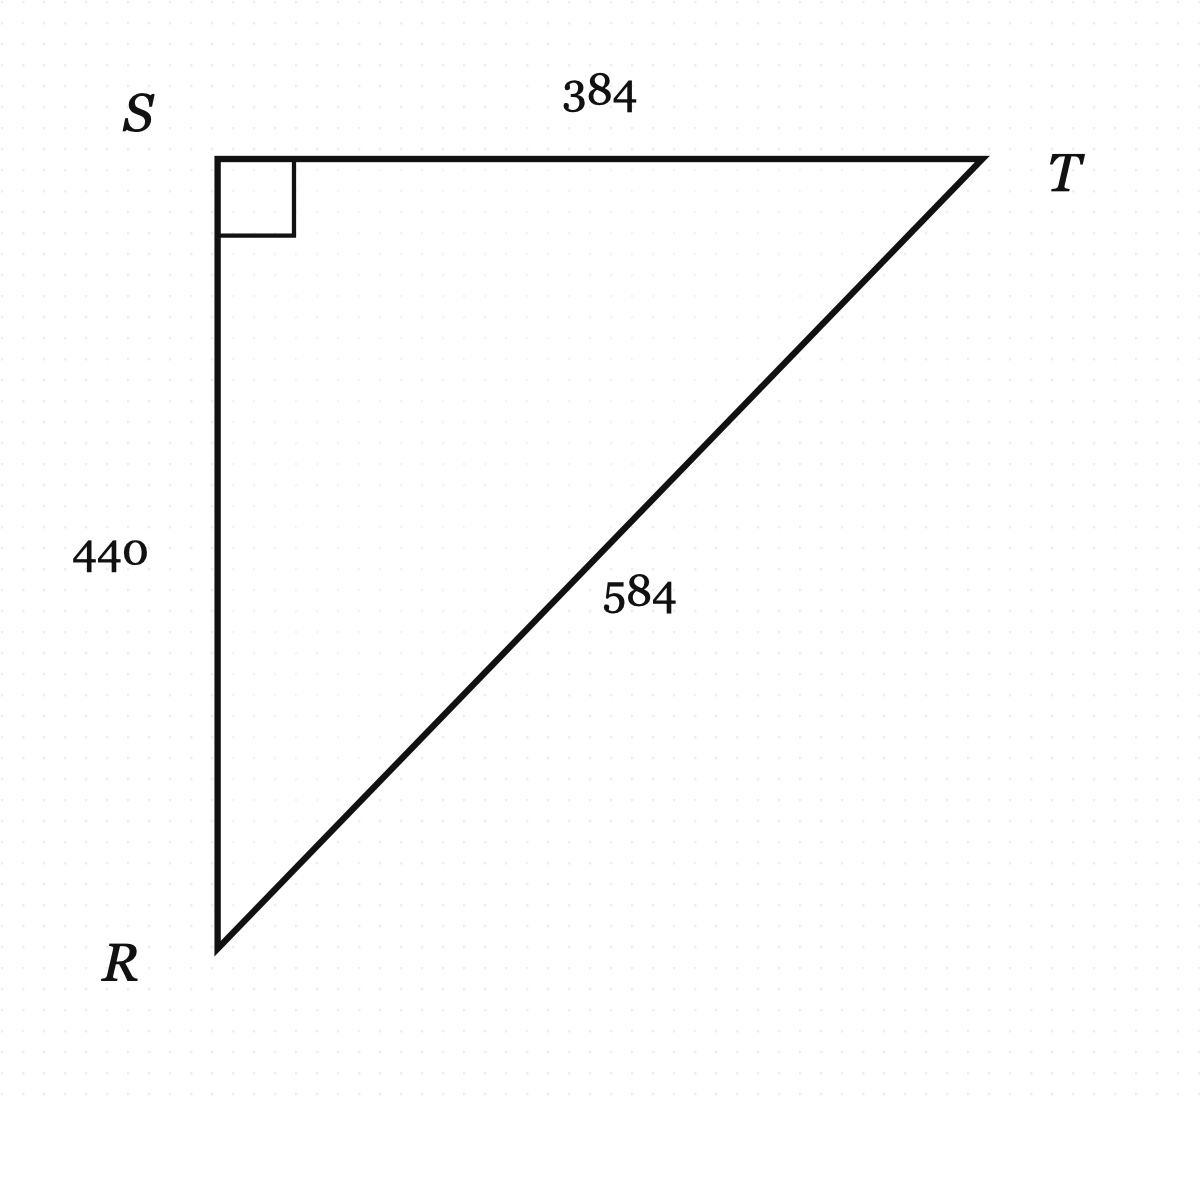
\includegraphics[width=0.64\linewidth]{rst_tri_440_384_584}
\end{center}

The side lengths of right triangle $RST$ are given.

\begin{align*}
RS &= 440 \\
ST &= 384 \\
TR &= 584
\end{align*}

Triangle $RST$ is similar to triangle $UVW$, where $S$ corresponds to $V$ and $T$ corresponds to $W$. What is the value of $\tan W$?
\begin{itemize}
    \item[\textbf{A.}] $\dfrac{48}{73}$
    \item[\textbf{B.}] $\dfrac{55}{73}$
    \item[\textbf{C.}] $\dfrac{48}{55}$
    \item[\textbf{D.}] $\dfrac{55}{48}$
\end{itemize}
\end{frame}
\begin{frame}{Answer: The side lengths of right triangle RST are given}
\textit{Strategy:} Similar triangles: $\tan W$ matches $\tan T$ (corresponding acute angles).

\textbf{Correct Answer:} \( \boxed{D} \)

\end{frame}
\begin{frame}{Question: A right triangle has legs with lengths of 24 centimeters and 21 centimet…}
A right triangle has legs with lengths of $24$ centimeters and $21$ centimeters. If the length of this triangle's hypotenuse, in centimeters, can be written in the form $3\sqrt{d}$, where $d$ is an integer, what is the value of $d$?
\end{frame}
\begin{frame}{Answer: A right triangle has legs with lengths of 24 centimeters and 21 centimet…}
\textit{Strategy:} $\sin 30^\circ=\dfrac{1}{2}$; use $30$-$60$-$90$ side ratios.

\textbf{Solution:}
\[ \boxed{113} \]
\textbf{Correct Answer:} \( \boxed{113} \)

\end{frame}
\begin{frame}{Question: The side lengths of right triangle RST are given}
\begin{center}
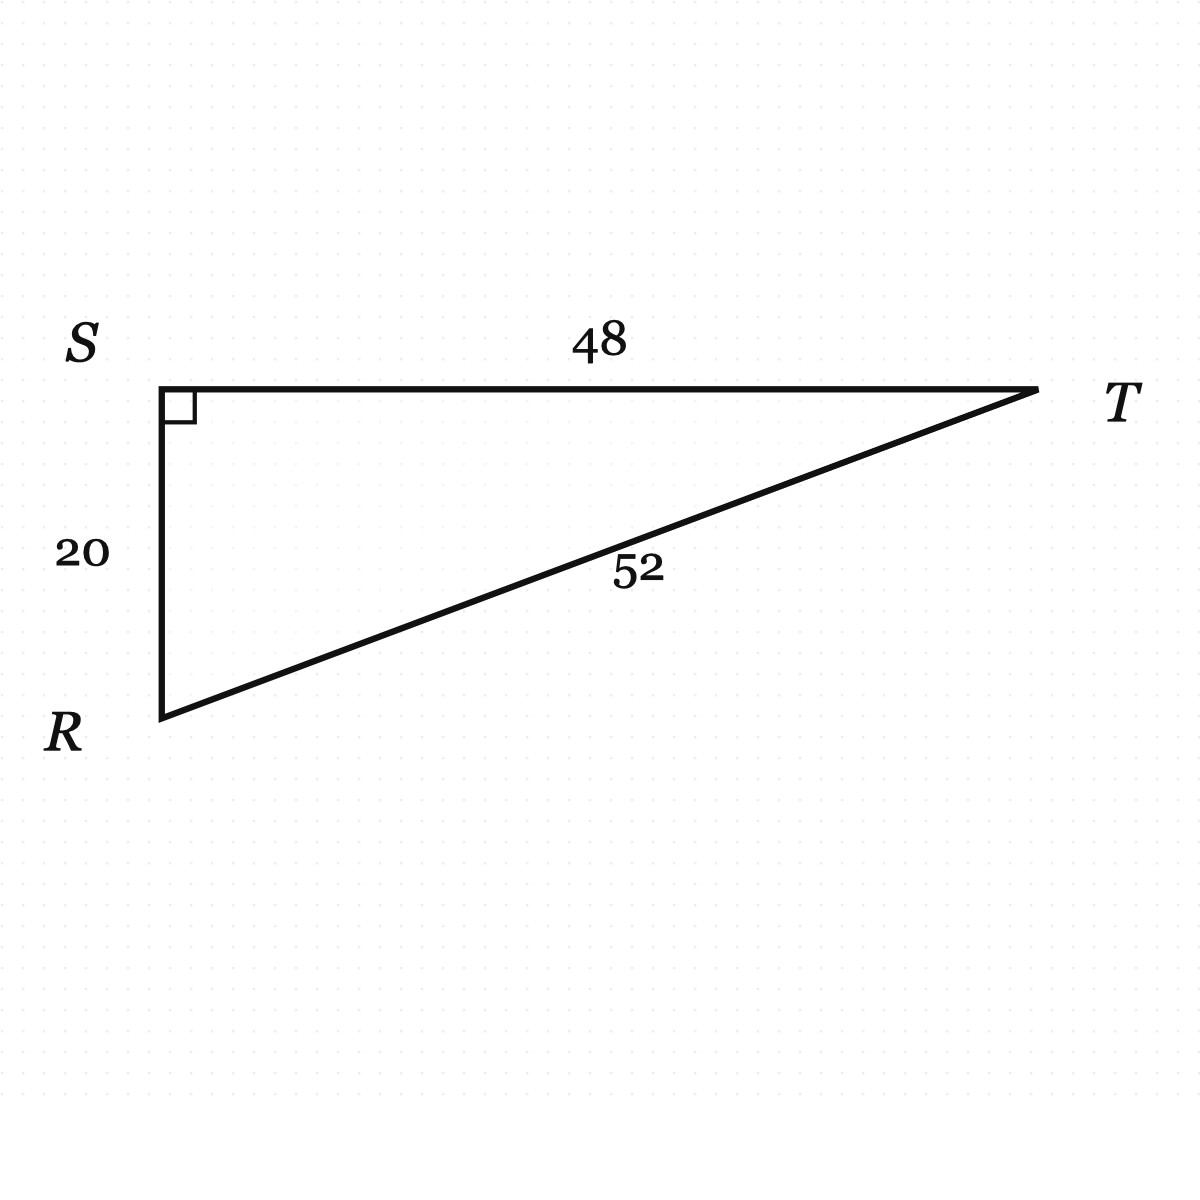
\includegraphics[width=0.64\linewidth]{rst_tri_20_48_52}
\end{center}

The side lengths of right triangle $RST$ are given.

\begin{align*}
RS &= 20 \\
ST &= 48 \\
TR &= 52
\end{align*}

Triangle $RST$ is similar to triangle $UVW$, where $S$ corresponds to $V$ and $T$ corresponds to $W$. What is the value of $\tan W$?
\begin{itemize}
    \item[\textbf{A.}] $\dfrac{5}{13}$
    \item[\textbf{B.}] $\dfrac{5}{12}$
    \item[\textbf{C.}] $\dfrac{12}{13}$
    \item[\textbf{D.}] $\dfrac{12}{5}$
\end{itemize}
\end{frame}
\begin{frame}{Answer: The side lengths of right triangle RST are given}
\textit{Strategy:} Complementary angles: $\sin A=\cos B$ when $A+B=90^\circ$.

\textbf{Correct Answer:} \( \boxed{B} \)

\end{frame}
\begin{frame}{Question: In triangle RST above, point W (not shown) lies on RT. What is the value…}
\begin{center}
    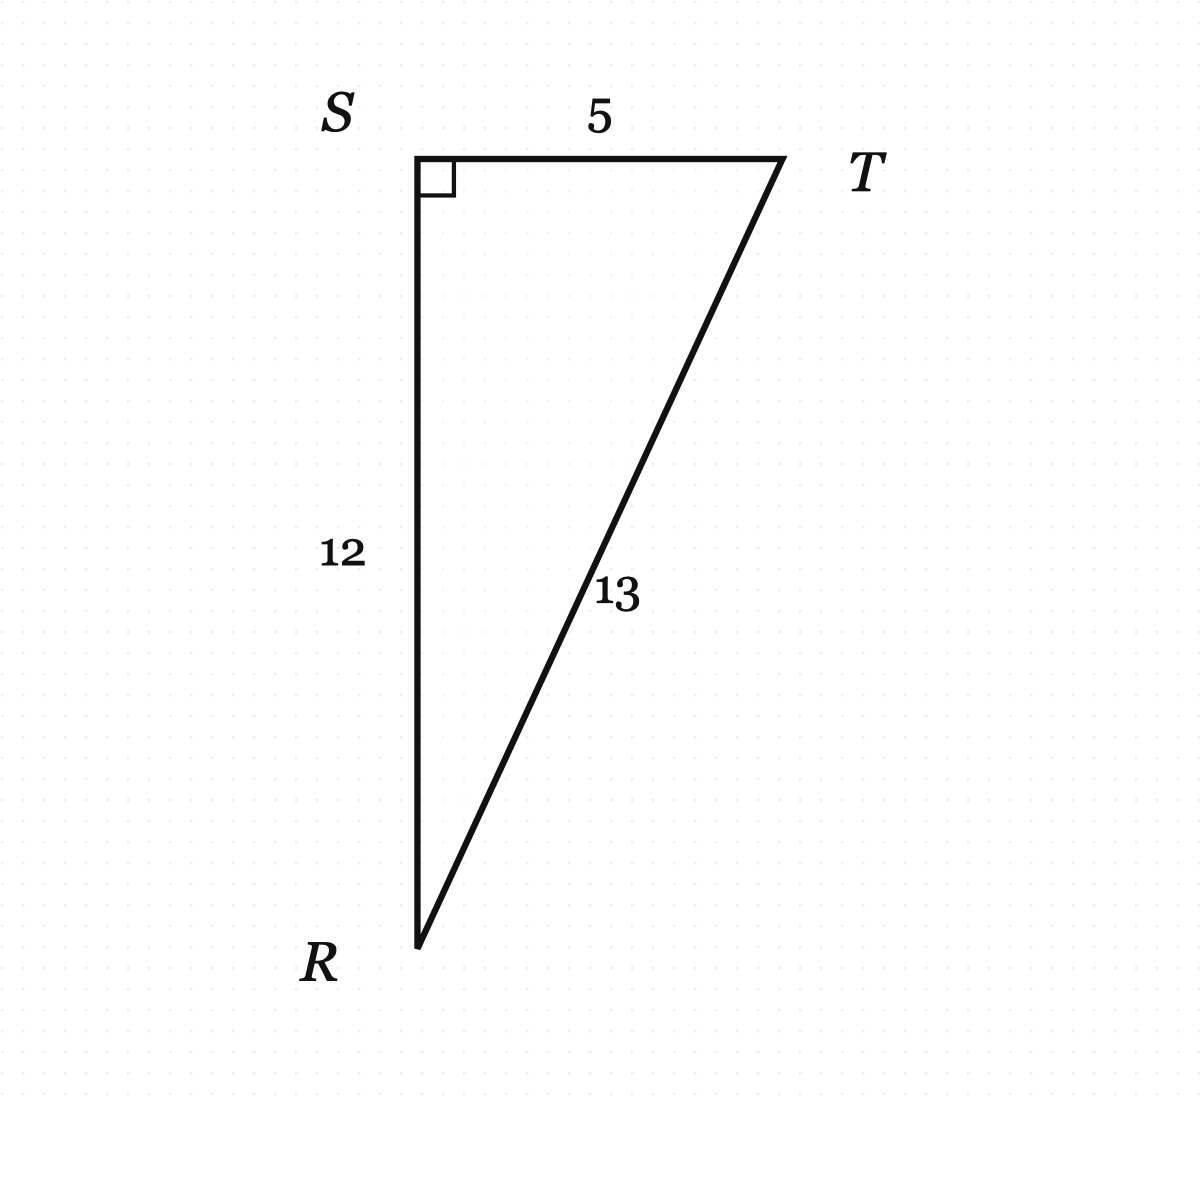
\includegraphics[width=0.76\linewidth]{rst_tri_12_5_13}
\end{center}

In triangle $RST$ above, point $W$ (not shown) lies on $\overline{RT}$. What is the value of $\cos(\angle RSW) - \sin(\angle WST)$?
\end{frame}
\begin{frame}{Answer: In triangle RST above, point W (not shown) lies on RT. What is the value…}
\textit{Strategy:} Pythagorean theorem to find the third side, then compute the ratio.

\textbf{Solution:}
\[ \boxed{0} \]
\textbf{Correct Answer:} \( \boxed{0} \)

\end{frame}
\begin{frame}{Question: Triangle ABC is similar to triangle DEF, where A corresponds to D and C …}
Triangle $ABC$ is similar to triangle $DEF$, where $A$ corresponds to $D$ and $C$ corresponds to $F$. Angles $C$ and $F$ are right angles. If $\tan(A) = \sqrt{3}$ and $DF = 125$, what is the length of $DE$?
\begin{itemize}
    \item[\textbf{A.}] $125\dfrac{\sqrt{3}}{3}$
    \item[\textbf{B.}] $125\dfrac{\sqrt{3}}{2}$
    \item[\textbf{C.}] $125\sqrt{3}$
    \item[\textbf{D.}] $250$
\end{itemize}
\end{frame}
\begin{frame}{Answer: Triangle ABC is similar to triangle DEF, where A corresponds to D and C …}
\textit{Strategy:} Similar right triangles share equal acute angles; trig ratios match.

\textbf{Correct Answer:} \( \boxed{D} \)

\end{frame}
\begin{frame}{Question: The length of a rectangle’s diagonal is 3 17, and the length of the rect…}
The length of a rectangle’s diagonal is $3\sqrt{17}$, and the length of the rectangle’s shorter side is $3$. What is the length of the rectangle’s longer side?
\end{frame}
\begin{frame}{Answer: The length of a rectangle’s diagonal is 3 17, and the length of the rect…}
\textit{Strategy:} $30$-$60$-$90$ or $\tan A=\sqrt{3}$ fixes the angle; use SOH-CAH-TOA on the similar triangle.

\textbf{Solution:}
\[ \boxed{12} \]
\textbf{Correct Answer:} \( \boxed{12} \)

\end{frame}
\begin{frame}{Question: A square is inscribed in a circle. The radius of the circle is 20 22 inc…}
A square is inscribed in a circle. The radius of the circle is $\dfrac{20\sqrt{2}}{2}$ inches. What is the side length, in inches, of the square?
\begin{itemize}
    \item[\textbf{A.}] $20$
    \item[\textbf{B.}] $\dfrac{20\sqrt{2}}{2}$
    \item[\textbf{C.}] $20\sqrt{2}$
    \item[\textbf{D.}] $40$
\end{itemize}
\end{frame}
\begin{frame}{Answer: A square is inscribed in a circle. The radius of the circle is 20 22 inc…}
\textit{Strategy:} Pythagorean theorem: $\text{longer}^2 = d^2 - 3^2$.

\textbf{Correct Answer:} \( \boxed{A} \)

\end{frame}
\begin{frame}{Question: Triangle ABC is similar to triangle DEF, where angle A corresponds to an…}
Triangle $ABC$ is similar to triangle $DEF$, where angle $A$ corresponds to angle $D$ and angles $C$ and $F$ are right angles. The length of $AB$ is $2.9$ times the length of $DE$. If $\tan A = \dfrac{21}{20}$, what is the value of $\sin D$?
\end{frame}
\begin{frame}{Answer: Triangle ABC is similar to triangle DEF, where angle A corresponds to an…}
\textit{Strategy:} A square inscribed in a circle has diagonal $=$ diameter $=2r$.

\textbf{Solution:}
\[ \boxed{0.7241} \]
\textit{Also accept: 21/29}
\textbf{Correct Answer:} \( \boxed{0.7241} \)

\end{frame}
\begin{frame}{Question: In a right triangle, the tangent of one of the two acute angles is 33. W…}
In a right triangle, the tangent of one of the two acute angles is $\dfrac{\sqrt{3}}{3}$. What is the tangent of the other acute angle?
\begin{itemize}
    \item[\textbf{A.}] $-\dfrac{\sqrt{3}}{3}$
    \item[\textbf{B.}] $-\dfrac{3}{\sqrt{3}}$
    \item[\textbf{C.}] $\dfrac{\sqrt{3}}{3}$
    \item[\textbf{D.}] $\dfrac{3}{\sqrt{3}}$
\end{itemize}
\end{frame}
\begin{frame}{Answer: In a right triangle, the tangent of one of the two acute angles is 33. W…}
\textit{Strategy:} Similar right triangles: $\sin D=\sin A$ when $A$ corresponds to $D$.

\textbf{Correct Answer:} \( \boxed{D} \)

\end{frame}
\begin{frame}{Question: Triangle ABC is similar to triangle DEF, where angle A corresponds to an…}
Triangle $ABC$ is similar to triangle $DEF$, where angle $A$ corresponds to angle $D$ and angle $C$ corresponds to angle $F$. Angles $C$ and $F$ are right angles. If $\tan(A) = \dfrac{50}{7}$, what is the value of $\tan(E)$?
\end{frame}
\begin{frame}{Answer: Triangle ABC is similar to triangle DEF, where angle A corresponds to an…}
\textit{Strategy:} Complementary acute angles: $\tan(90^\circ-\theta)=\dfrac{1}{\tan\theta}$.

\textbf{Solution:}
\[ \boxed{7/50} \]
\textbf{Correct Answer:} \( \boxed{7/50} \)

\end{frame}
\begin{frame}{Question: In the figure above, BD is parallel to AE. What is the length of CE?}
\begin{center}
    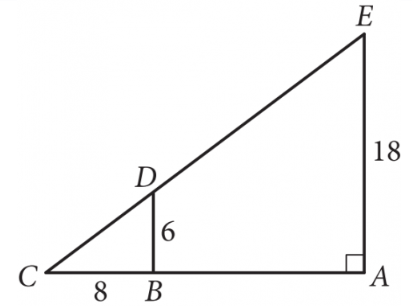
\includegraphics[width=0.56\linewidth]{22.png}
\end{center}

In the figure above, $\overline{BD}$ is parallel to $\overline{AE}$. What is the length of $\overline{CE}$?
\end{frame}
\begin{frame}{Answer: In the figure above, BD is parallel to AE. What is the length of CE?}
\textit{Strategy:} Parallel lines create similar triangles; set up a proportion for $CE$.

\textbf{Solution:}
\[ \boxed{30} \]
\textbf{Correct Answer:} \( \boxed{30} \)

\end{frame}
\begin{frame}{Question: In triangle JKL, (K) = 24/51 and angle J is a right angle. What is the v…}
In triangle $JKL$, $\cos(K) = \dfrac{24}{51}$ and angle $J$ is a right angle. What is the value of $\cos(L)$?
\end{frame}
\begin{frame}{Answer: In triangle JKL, (K) = 24/51 and angle J is a right angle. What is the v…}
\textit{Strategy:} Draw a right triangle for $\cos K$; use Pythagorean theorem for adjacent side.

\textbf{Solution:}
\[ \boxed{15/17} \]
\textbf{Correct Answer:} \( \boxed{15/17} \)

\end{frame}
\begin{frame}{Question: A triangle with angle measures 30°, 60°, and 90° has a perimeter of 18 +…}
A triangle with angle measures $30^\circ$, $60^\circ$, and $90^\circ$ has a perimeter of $18 + 6\sqrt{3}$. What is the length of the longest side of the triangle?
\end{frame}
\begin{frame}{Answer: A triangle with angle measures 30°, 60°, and 90° has a perimeter of 18 +…}
\textit{Strategy:} $30$-$60$-$90$ triangle side ratio $1:\sqrt{3}:2$.

\textbf{Solution:}
\[ \boxed{12} \]
\textbf{Correct Answer:} \( \boxed{12} \)

\end{frame}

\begin{frame}{}
    \begin{tikzpicture}[remember picture, overlay]
        \shade[top color=novelPurple!40, bottom color=white]
            (current page.north west) rectangle (current page.south east);
        \fill[white, opacity=0.15] (current page.center) circle (5cm);
        \foreach \x in {1,2,3,4,5} {
            \fill[novelPurple, opacity=0.12] (rand*10-5, rand*7-3.5) circle (0.1+\x*0.05);
        }
    \end{tikzpicture}
    \centering
    \vspace{5em}
    {\Huge \textbf{\textcolor{novelPurple}{Thank You!}}} \\[1em]
    {\large \textcolor{gray}{We appreciate your time and focus.}} \\[3em]
    {\LARGE \textbf{\textcolor{novelPurple}{\textsf{Novel Prep}}}}
    \vfill
\end{frame}

\end{document}
